% !TEX TS-program = xelatex
% !TEX encoding = UTF-8 Unicode
% !TEX spellcheck = ru-RU
% !BIB program = biber

\documentclass[a4paper,14pt]{extarticle} % ext for 14 font

\usepackage{etoolbox}
\newbool{comicsans}
\boolfalse{comicsans}

%!TEX root = thesis.tex

\usepackage[english,russian]{babel}	% локализация и переносы
\usepackage{fontspec}
\ifbool{comicsans}{
	\setmainfont{Comic Sans MS}
}{
	\setmainfont{Times New Roman}
}
%\usepackage{tempora} % font for not xelatex

%\tolerance=1
%\emergencystretch=\maxdimen
%\hyphenpenalty=10000
%\hbadness=10000
\hyphenchar\font=-1
\sloppy

\usepackage{graphicx}
\usepackage{geometry}
	\geometry{left=2cm}
	\geometry{right=1cm}
	\geometry{top=2cm}
	\geometry{bottom=2cm}

\usepackage{setspace}
	\onehalfspacing

\setlength{\parindent}{1.25cm} % paragraph indent
\usepackage{indentfirst}
\setlength{\parskip}{0cm} % paragraph skip
\usepackage{titlesec}
\titlespacing*{\section}{\parindent}{*1}{*1}
\titlespacing*{\subsection}{\parindent}{*1}{*1}
\titlespacing*{\subsubsection}{\parindent}{*1}{*1}

\usepackage{multicol}
\usepackage{multirow}
\usepackage{tabularx}
\usepackage{makecell}

\newcommand{\titlefont}{\fontsize{18}{21.6}\bfseries\hyphenchar\font=-1}
\usepackage{titlesec}
\titleformat{\section}[block]
{\titlefont} {\thesection}{1em}{}
\titleformat{\subsection}[block]
{\titlefont} {\thesubsection}{1em}{}
\titleformat{\subsubsection}[block]
{\titlefont} {\thesubsubsection}{1em}{}
\newcommand{\centertitle}[1]{
	\setlength\parskip{0pt}
	\begin{center}
		\setlength\parskip{1ex}
		{\titlefont \uppercase{#1}}
	\end{center}
}
\newcommand{\centertitletoc}[1]{
	\setlength\parskip{0pt}
	\begin{center}
		{\titlefont \uppercase{#1}}
		\phantomsection
		\addcontentsline{toc}{section}{#1}
	\end{center}
}

\usepackage{caption}
\DeclareCaptionFont{captionsize}{\fontsize{13}{15.6}\selectfont}
\captionsetup{
	font=captionsize,
	justification=centering,
	labelsep=period,
	figurewithin=none,
	tablewithin=none,
	margin=1cm
}
\captionsetup[table]{
	justification=RaggedLeft,
	singlelinecheck=false,
	labelsep=newline,
	margin=0cm,
	skip=4pt
}
\usepackage{float}

\usepackage{tocloft} % toc style
\setlength{\cftsecnumwidth}{0pt}
\renewcommand{\cftsecaftersnumb}{\hspace{1.5em}}

\newcommand{\ris}[1]{(рис.~#1)}

\usepackage[
	backend=biber,
	sorting=none,
	style=gost-numeric
]{biblatex}
\addbibresource{mendeley.bib}

\usepackage{hyperref}
\hypersetup{				% Гиперссылки
	unicode=true,           % русские буквы в разделах PDF
	pdftitle={Разработка системы контроля и управления энергопотреблением элементов графического интерфейса на мобильных устройствах},   % Заголовок
	pdfauthor={Юндин Владислав},      % Автор
	colorlinks=true,       	% false: ссылки в рамках; true: цветные ссылки
	linkcolor=black,          % внутренние ссылки
	urlcolor=black,
	citecolor=black,        % на библиографию
}

\addto\captionsrussian{%
	\renewcommand{\contentsname}%
	{Оглавление}%
}

\usepackage{pdfpages}

\begin{document}
	%!TEX root = thesis.tex

\thispagestyle{empty}
\newgeometry{left=2cm,right=2cm,top=1.25cm,bottom=1.25cm}
\begin{center}
    \small
    ФЕДЕРАЛЬНОЕ ГОСУДАРСТВЕННОЕ АВТОНОМНОЕ ОБРАЗОВАТЕЛЬНОЕ \\ УЧРЕЖДЕНИЕ ВЫСШЕГО ОБРАЗОВАНИЯ \\ 
    «НАЦИОНАЛЬНЫЙ ИССЛЕДОВАТЕЛЬСКИЙ УНИВЕРСИТЕТ \\ 
    «ВЫСШАЯ ШКОЛА ЭКОНОМИКИ» \\
        
    \vspace{5mm}
    
    МОСКОВСКИЙ ИНСТИТУТ ЭЛЕКТРОНИКИ И МАТЕМАТИКИ \\
    им. А.Н. ТИХОНОВА
    
    \normalsize
    \vspace{12mm}
    
    Юндин Владислав Андреевич
    
    \vspace{12mm}
    
    \textbf{РАЗРАБОТКА СИСТЕМЫ КОНТРОЛЯ И УПРАВЛЕНИЯ ЭНЕРГОПОТРЕБЛЕНИЕМ ЭЛЕМЕНТОВ ГРАФИЧЕСКОГО ИНТЕРФЕЙСА НА МОБИЛЬНЫХ УСТРОЙСТВАХ}
    
    \vspace{8mm}
    
    Выпускная квалификационная работа по направлению подготовки \\ 
    09.03.01. Информатика и вычислительная техника \\
    студента образовательной программы \\
    <<Информатика и вычислительная техника>>
\end{center}

\vspace{10mm}

\begin{multicols}{2}
    \noindent
    \textbf{Студент}
    
    \vspace{4mm}
    
    \noindent
    \begin{tabularx}{\linewidth}{Xc}
        & / В.А. Юндин \\
        \hline
    \end{tabularx}
    
    \columnbreak
    
    \noindent
    \textbf{Руководитель}
    
    \vspace{4mm}
    
    \noindent
    \begin{tabularx}{\linewidth}{c}
        должность, звание, А.Ю. Ролич \\
        \hline
    \end{tabularx}

    \vspace{8mm}

    \noindent
    \textbf{Консультант}
    
    \vspace{4mm}
    
    \noindent
    \begin{tabularx}{\linewidth}{c}
        должность, звание, И.О. Фамилия \\
        \hline
    \end{tabularx}

    \vspace{8mm}
    
    \noindent
    \textbf{Рецензент}
    
    \vspace{4mm}
    
    \noindent
    \begin{tabularx}{\linewidth}{c}
        должность, звание, И.О. Фамилия \\
        \hline
    \end{tabularx}
\end{multicols}

\vfill
\begin{center}Москва, 2020\end{center}

\restoregeometry
\newpage

	\centertitle{Задание на ВКР}
	\centertitle{График выполнения ВКР}
	\centertitle{Аннотация на русском языке}
	\centertitle{Аннотация на английском языке}
	
	\newpage
	\tableofcontents
	\newpage
	
	%!TEX root = thesis.tex

\centertitletoc{Введение}

Современная жизнь немыслима без смартфонов и разных мобильных приложений, которые могут неэффективно потреблять ресурсы устройства. Значительные проблемы в оптимизации пользовательского опыта возникают в вопросах разряда батареи. Энергоэффективность приложений --- одна из важнейших проблем, с которой сталкиваются как разработчики, так и пользователи~\parencite{man2016experience, wasserman2010software}. Низкая энергоэффективность приложения ускоряет разрядку смартфона и может даже стать основанием для удаления приложения~\parencite{ickin2017users}. Данная проблема имеет популярность среди исследователей, и является предметом большого количества работ. Предложено множество способов снижения энергопотребления, но мне хотелось бы проверить эффективность метода, который основан на замене менее эффективных виджетов на экране более эффективными.

\subparagraph{Цель и задачи}
Конечной целью выпускной квалификационной работы является разработка системы контроля и управления энергопотреблением элементов графического интерфейса на устройствах под управлением операционной системы Android. Для её достижения необходимо решить следующие задачи:
\begin{itemize}
	\item Проанализировать существующие исследования по оптимизации энергопотребления;
	\item Определить инструменты для измерения энергопотребления Android-смартфонов;
	\item Измерить энергопотребление различных элементов пользовательского интерфейса;
	\item Создать библиотеку для мониторинга и управления энергопотреблением графических элементов пользовательского интерфейса
\end{itemize}

\subparagraph{Практическая значимость}
Решение данной проблемы в первую очередь представляет интерес для тех, кто занимается разработкой приложений для Android. Любой инженер, которому важно количество потребляемой приложением энергии, сможет встроить библиотеку в приложение для выявления наиболее затратных элементов интерфейса. Также, полученная библиотека составит список рекомендаций по снижению нагрузки на аккумулятор устройства. Благодаря созданной библиотеке, будет увеличено время автономной работы устройств пользователей.

\subparagraph{Программные средства}
Для разработки системы будет использован язык программирования Kotlin, фреймворк автоматического тестирования пользовательского интерфейса Kaspresso, а также инструмент анализа информации энергопотребления Battery Historian.
	
	\newpage
	\section{Актуальность работы}
	
	Смартфон — неотъемлемая часть жизни современного человека. Человек может использовать телефон до 200 раз каждый день [1]. Тем не менее, смартфоны всё ещё не достигли потолка своего развития и многие аспекты нуждаются в улучшении. Одним из таких является энергопотребление устройства.
	
	Проблема заключается в том, что с развитием вычислителей и экранов, которые потребляют всё больше энергии, аккумуляторы должны развиваться с сопоставимой скоростью, чтобы покрыть растущие затраты и оставить время работы устройства от батареи хотя бы на том же уровне. Но развитие аккумуляторов устройств происходит не так быстро [2], что заставляет задуматься о более эффективном расходовании уже имеющейся энергии.
	
	Раньше мобильные телефоны могли работать более недели от одного заряда аккумулятора, но с их развитием такая возможность была потеряна. Как видно на диаграмме (рис. 1), процесс увеличения числа возможностей портативных устройств сопряжён с уменьшением времени работы прибора. Если в 1996 году портативное устройство было способно работать 8-10 недель до разрядки аккумулятора, то уже в 2004 году наличие камеры, диктофона, Bluetooth, цветного дисплея и другой функциональности сократили время работы до недели и меньше [3].
	
	Имеют место большое количество факторов, которые влияют на потребление энергии. Это взаимодействие с сетью, множество сенсоров и датчиков, камера, экран и другие. Существуют академические работы, показывающие возможность оптимизировать потребление многих факторов, например, взаимодействие с интернетом [4] или более оптимальное использование оперативной памяти может продлить срок работы устройства от аккумулятора [5]. Но также исследования показывают, что в большинстве сценариев использования смартфона энергозатраты на экран составляют больше половины всех энергозатрат [6]. Становится очевидным, что именно потребление экрана нуждается в оптимизации в первую очередь.
	
	Существует множество подходов к уменьшению потребления экрана, которые основываются на самых разных идеях. Некоторые считают, что изменение цветовой схемы интерфейса на AMOLED экранах поможет снизить затраты [7], другие понижают кадровую частоту и частоту обновления экрана [8, 9]. 
	
	Новизна моего исследования базируется на предположении, что взаимозаменяемые виджеты со схожей функциональностью потребляют разное количество энергии, что позволяет заменить более затратные виджеты на аналогичные и уменьшить энергопотребление.
	
	Практическое применение моей работы заключается в помощи разработчикам Android-приложений в выборе наиболее эффективных элементов графического интерфейса и улучшение общего качества приложения. Ожидается, что этого удастся достигнуть путём непрерывного сканирования иерархии виджетов с целью поиска тех, которые могут быть заменены на более оптимальные, и сообщения об этом разработчику мобильного приложения.
	
	\newpage
	\section{Обзор литературы} % Анализ существующих технических решений объекта разработки
	
	В этой главе я рассмотрю работы, затрагивающие проблему энергопотребления мобильных устройств, и предлагающие пути её решения. Это необходимо для понимания проделанной  исследователями работы, а также изучения методик и инструментов, используемых для проведения измерений.
	
	\subsection{Проблемы пользователей и разработчиков мобильных приложений}
	
	Я считаю необходимым иметь представление о реальных проблемах мобильных приложений как по мнению пользователей, так и понимать проблемы, стоящие перед разработчиками приложений. Это поможет правильно расставить приоритеты исследования и разработать наиболее удобное и полезное решение по контролю энергопотребления.
	
	Одна из проблем, освещённая в статье Мана, Гао и др., связана с пользовательским восприятием приложений [10]. Авторами был создан новый фреймворк под названием CrossMiner для автоматического анализа проблем приложений из отзывов пользователей с помощью метода, основанного на ключевых словах. Основываясь на пяти миллионах отзывов пользователей, платформа автоматически фиксирует распределение семи проблем приложения, а именно: “батарея”, “сбой”, “память”, “сеть”, “конфиденциальность”, “спам” и “пользовательский интерфейс”. По итогу было выявлено, что проблемы, связанные со “сбоем” и “сетью”, больше беспокоят пользователей, чем другие проблемы на трех рассматриваемых платформах (Google Play, App Store и Windows Store).
	
	\begin{figure}[h]
		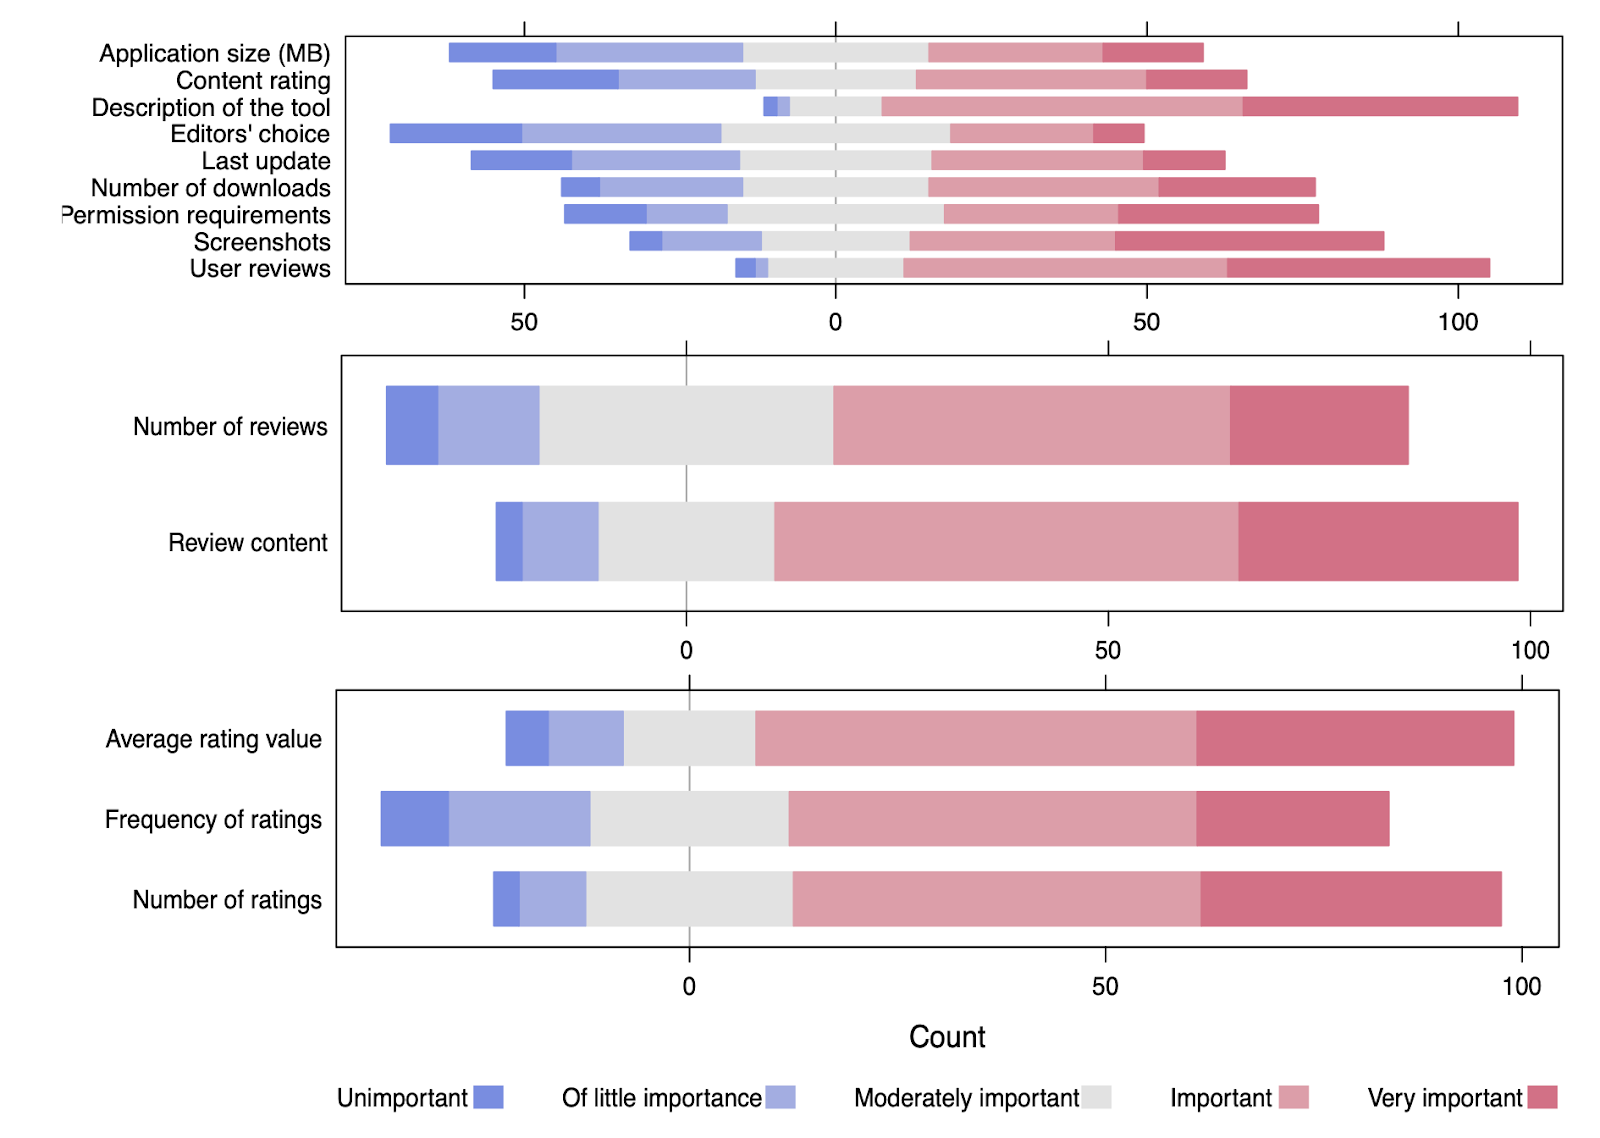
\includegraphics[width=\textwidth]{install_reasons}
		\caption{Причины установки приложений пользователями}
		\label{fig:install_reasons}
	\end{figure}
	
	В другой работе задача состояла в том, чтобы определить причины, по которым пользователи выбирают и устанавливают мобильные приложения из магазинов приложений [11]. А также причины, по которым пользователи удаляют приложения. Было проведено анкетирование с участием 121 пользователя из 26 различных стран. Как видно на диаграмме \ris{\ref{fig:install_reasons}}, самыми частыми причинами установки приложения являются его описание, оценки пользователей и скриншоты приложения. Согласно другим данным \ris{\ref{fig:delete_reasons}} в топе причин удаления — бесполезность, сбои, высокое использование оперативной памяти.

	\begin{figure}[h]
		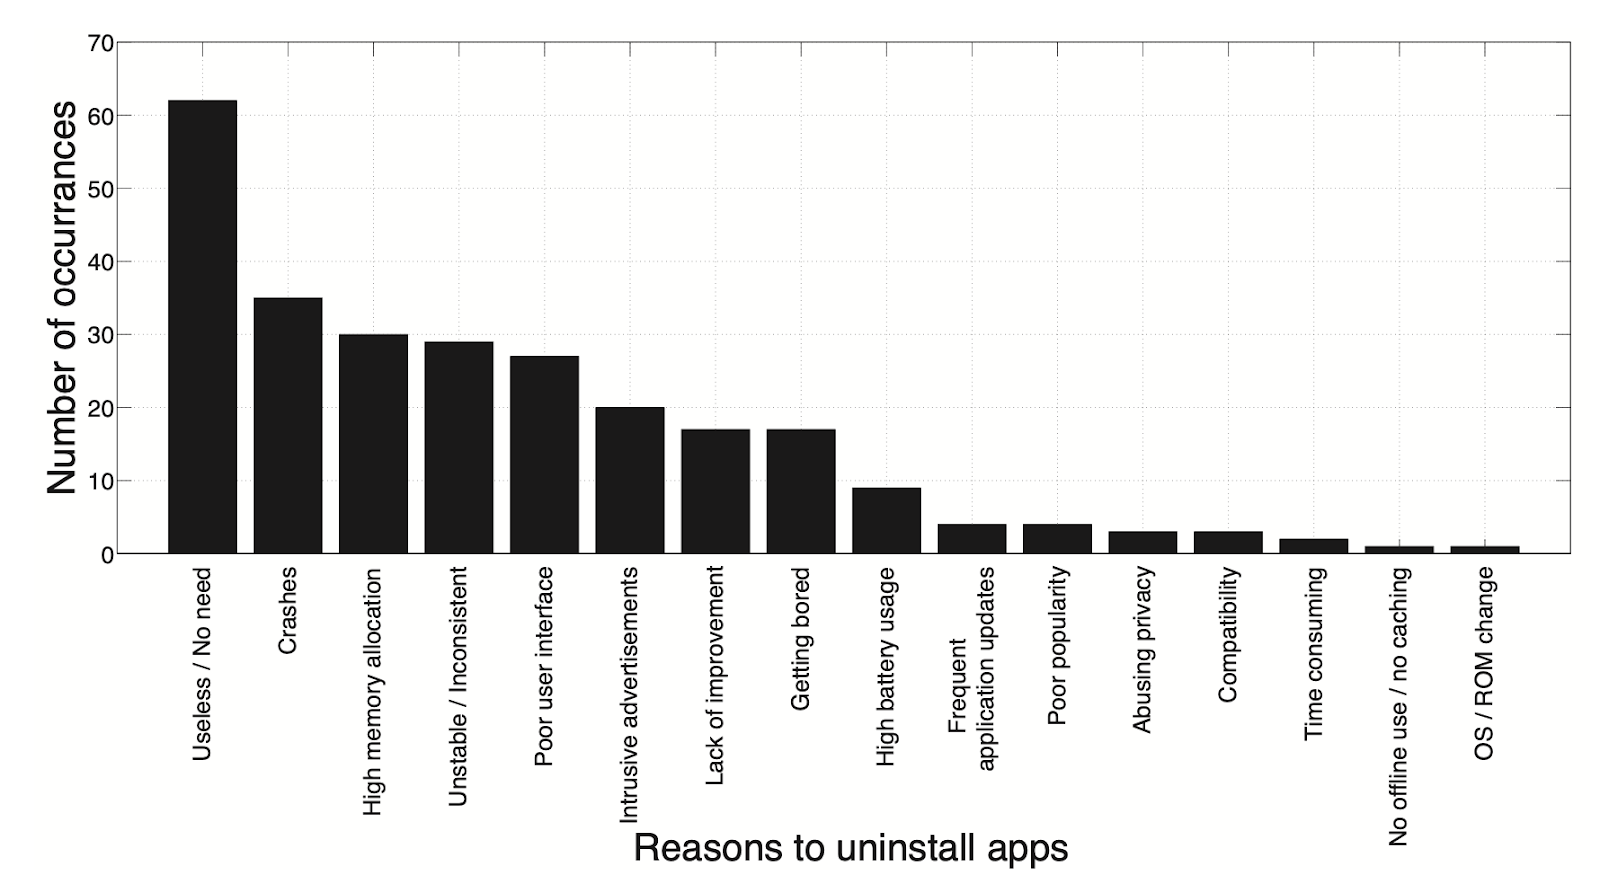
\includegraphics[width=\textwidth]{delete_reasons}
		\caption{Причины удаления приложений пользователями}
		\label{fig:delete_reasons}
	\end{figure}
	
	С точки зрения инженеров [12] наиболее остро стоят следующий вопросы: 
	\begin{itemize}
		\item Улучшение пользовательского опыта; 
		\item Нефункциональные требования (производительность, энергоэффективность, надёжность, качество, безопасность);
		\item Процессы, инструменты и архитектура; 
		\item Переносимость на другие платформы. 
	\end{itemize}

	Эти пункты являются лишь подмножеством возможных тем исследований в области разработки программного обеспечения для мобильных приложений, но служат для обозначения широты исследовательских потребностей и возможностей в этой формирующейся области.
	
	\subsection{Измерение энергопотребления устройств}

	Как мы выяснили ранее, понимание энергопотребления компонентов смартфона является одной из ключевых областей интереса для конечных пользователей, а также разработчиков приложений и системного программного обеспечения. Существующая литература предлагает множество решений для эффективного измерения энергопотребления, что помогает определить влияние различных подходов к оптимизации.

	Группа исследователей представила «двухэтапный способ оценки влияния работы приложений и их функций на энергопотребление в некотором самостоятельном “устройстве” с автономным источником питания при помощи отдельной “основной системы” с использованием линейной математической модели» [13]. Данный подход позволяет определять наиболее энергозатратные участки кода и проводить оптимизацию ПО. Всё это в конечном счёте продлевает время автономной работы мобильных устройств. 
	
	В другой работе был предложен программный инструмент, использующий технологии параллельного программирования OpenMP и Cilk Plus [14]. В серии экспериментов они оказались более энергоэффективными, чем последовательные реализации. Архитектура системы обеспечивает ее расширяемость, позволяя добавлять новые источники данных, метрики и способы визуализации, что значительно выделяет разработку среди остальных.
	
	В зарубежных исследованиях также можно отметить тенденцию предложения использования конкретного инструментария, которые предлагают сами авторы работы. Так, в департаменте компьютерных наук университета Ёнсе в Южной Корее, был разработан AppScope — приложение для автоматического измерения энергопотребления приложений Android с помощью мониторинга активности ядра [15]. Оно отслеживает системные вызовы, а также анализирует данные механизма IPC операционной системы . 
	
	Проектная группа из университета Джорджа Мейсона и Национального института стандартов и технологий США представила систему, которая эффективно учитывает энергопотребление всех основных аппаратных подсистем телефона: процессора, дисплея, графики, GPS, аудио, микрофона и Wi-Fi [16]. Для этого они использовали доли времени для каждой подсистемы, сообщаемые модулем управления питанием операционной системы. Предложенное решение позволяет работать в режиме реального времени без значительного влияния на энергопотребление подконтрольного устройства, что может помочь разработчикам принять более оптимальные решения для повышения энергоэффективности.
	
	\subsection{Энергопотребление при взаимодействии с сетью}
	
	При рассмотрении энергопотребления мобильных устройств в целом, стоит обратить особое внимание на беспроводные коммуникации, поскольку они потребляют значительную часть общей энергии системы. Также методы измерения и оптимизации потребления сетевых модулей могут быть позднее использованы и для других модулей устройства.
	
	Б. В. Окунев и И. А. Жужгина предлагают сократить энергозатраты во время с работы беспроводными Wi-Fi сетями, сохранив возможности пользователей по управлению ресурсами, с помощью особой процедуры поиска и подключения к точкам доступа [17]. На первоначальном этапе производится поиск доступных беспроводных сетей в радиусе действия. В дальнейшем пользователю предоставляется возможность выбора сети из списка. После подключения к выбранной пользователем сети циклический поиск других доступных сетей больше не производится до того момента, пока этого не пожелает пользователь.
	
	В другой статье рассмотрен энергосберегающий алгоритм работы мобильных устройств с беспроводными самоорганизующимися Wi-Fi-сетями (Ad-hoc) [18]. Он предназначен для использования в мобильных устройствах, работающих на основе операционной системы Android, и позволяет уменьшить в среднем на 10\% энергопотребление смартфона при прочих равных условиях.
	
	Компания Redpine Signals представила разработку, позволяющую обеспечить высокоскоростной обмен данными при исключительно низкой потребляемой мощности [19]. Теоретическое быстродействие современного стандарта IEEE 820.11n позволяет достигать быстродействия до 300 Мбит/с при условии применения пространственного мультиплексирования и нескольких приемных и передающих антенн. Снижение показателей энергопотребления в свою очередь было достигнуто благодаря улучшенной системе управления питанием устройства.
	
	Также стоит упомянуть профилировщик энергопотребления сети в режиме реального времени и инструмент выбора сети или интерфейса с учетом энергопотребления для смартфонов на базе Android [20]. Инструмент был опубликован в магазине Google Play. Предложенное решение сообщает об уровнях энергопотребления различных сетевых интерфейсов (Wi-Fi и сотовой связи), используя фактические измерения пакетов и точные вычисления, и позволяет устройствам осуществлять передачу обслуживания горизонтально/вертикально для повышения энергоэффективности.

	\subsection{Оптимизации на уровне исходного кода}

	Одним из инновационных подходов к снижению потребления энергии устройством является оптимизация затрат процессорного времени, которое требуется для выполнения вычислительных задач. В данной главе будут рассмотрены пути оптимизации исходного кода программы с целью сокращения времени нагруженной работы процессора и скорейшего его перехода в энергосберегающий режим.
	
	Исследование показало, что JavaScript экономит больше энергии и работает медленнее, чем другие подходы, и что гибридизация приложений может быть решением для оптимизации приложений как с точки зрения производительности, так и энергопотребления [21]. Среди двух вариантов гибридизации использование NDK является наиболее безопасным вариантом для повышения производительности, но использование веб-подхода может дать лучший результат при небольшом количестве кросс-языковых вызовов.
	
	В статье Сео, Малека и Медвидовика представлена структура для оценки энергопотребления программных систем на основе Java [22]. Её инфраструктура явно использует компонентную перспективу, что делает ее подходящей для большого класса современных распределенных, встроенных и распространяющихся приложений. В большом количестве сценариев распределенных приложений платформа показала очень хорошую точность в целом, давая результаты, которые были в пределах 5\% от фактического потребления энергии, понесенного при выполнении программного обеспечения. 
	
	Ещё одно исследование относительно Java сфокусировано вокруг сжатия — одного из популярных механизмов для снижения требований систем к памяти [23]. В статье рассматривается влияние сжатия на использование системных ресурсов встроенной виртуальной машиной Java (JVM), а также алгоритмы сжатия. Опыты показали, что экономия энергии составляет в среднем 21\%. В двух приложениях, где декомпрессия играет большую роль, результаты получаются хуже, чем в случае оригинала.
	
	Необычный подход использован в работе И. П. Токаря по поиску техник компиляции, повышающих энергоэффективность программ [24]. Программа рассматривается, как состоящая из регионов (где каждой функции соответствует максимум один регион), каждый из которых исполняется на разной частоте процессора, а, следовательно, имеет разное напряжения питания, потребление энергии и производительность.
	
	Для решения этой задачи предлагается и реализуется генетический алгоритм, который находит частоты для каждого региона, обеспечивающие максимальную энергоэффективность, при этом сохраняя производительность в заданных пользователем рамках. Приводятся результаты измерения его эффективности на физическом устройстве. Достигается 13,5\% роста энергоэффективности на некоторых тестах из пакета SPEC2000 (в частности 183.equake). Главным недостатком данного алгоритма является неспособность взаимодействовать с операционной системой и другими процессами в многоядерных системах.
	
	\subsection{Методы оптимизации потребления ресурсов в портативных устройствах}
	
	Многие проблемы энергопотребления приходилось решать ранее для оптимизации различных портативных устройств. Разработанные методы можно применить и для улучшения энергоэффективности смартфонов. 
	
	В статье Маурицио предлагается глобально пересмотреть подход к производству с учетом интересов конечного пользователя [25]. А именно: изменить подбор архитектуры и уделять внимание экономии энергии на каждой стадии разработки продукта. При выборе архитектуры автор предлагает учитывать критерий энергопотребления, например, энергозатратные архитектуры, использующие ТПЛ и дифференциальные сигнальные методы со скоростью передачи данных более 10 Гбит/с, должны быть тщательно сопоставлены с менее энергоемкими методиками, такими как КМОП и использование несимметричных архитектур. В дополнение к данному подходу делается акцент на необходимости дальнейшей оптимизации уже существующих архитектур, дополняя их новыми характеристиками.
	
	В другой статье возлагаются большие надежды на открытие нового типа электрохимической системы аккумуляторной батареи или усовершенствование старой, а также экономию энергии за счет применения интеллектуальных микросхем управления питания [26].
	
	Анализ энергопотребления и средней задержки для типового режима энергосбережения с несколькими циклами ожидания показал, что можно подбирать оптимальные параметры режимов ожидания с учетом ограничения средней начальной задержки [27]. Предложенная автором методика базируется на простой математической модели входного потока, которая применима и для сложных систем с большим числом состояний. Критерием её применимости является условие, при котором функционирование системы можно разбить на циклы регенерации.
	
	Также можно рассмотреть более частные случаи. Например, способы по оптимизации потребления энергии устройствами, основным элементом которых является микроконтроллер. Они нашли себе применение в том числе и в смартфонах. Обзор охватывает программные, архитектурные и схемотехнические способы снижения потребления [28].
	
	Программные способы направлены на снижение вычислительной нагрузки на микропроцессор. Приведены такие способы, как использование специфичной математики, так как операции с дробными числами занимают продолжительное время. Также учёт разрядности процессора может сыграть существенную роль в снижении энергопотребления. Ещё один способ предполагает переписывание критичных участков кода на язык ассемблера, но это поставит крест на кроссплатформенности получившихся решений.
	
	Архитектурные способы применяются разработчиками микроконтроллера и к ним относится реализация различных режимов энергосбережения, что позволяет отключать неиспользуемую перифирию, а также снижать тактовую частоту процессора. Также отключение неиспользуемых узлов кристалла позволит в разы снизить потребление энергии.
	
	Схемотехнические методы оптимизации применимы к самой аккумуляторной батарее. Предлагается использование литий-ионных или литий-полимерных источников питания для обеспечения прямого питания схемы от батареи. Также предлагается различное напряжение питания для вычислительного ядра и периферии, но это приводит к снижении тактовой частоты микросхем.
	
	Альтернативный взгляд на проблему — признание важности влияния ПО на потребление энергии нижележащим аппаратным обеспечением. В работе А. В. Юрченко применяются иерархические энергетические меры, получаемые из граф-схемы программы [29]. Они использованы для определения количества выполненных инструкций и количества операций доступа к памяти данных. Основываясь на полученных мерах, были определены программные метрики энергоэффективности, используемые для оценки энергопотребления процессора и операций доступа к памяти данных и памяти команд. В дальнейшем необходимо определить более подробные, сложные метрики, которые помогли бы разработчикам создавать более качественное ПО в терминах энергопотребления.
	
	\subsection{Энергопотребление в операционной системе Android}

	Следующая предметная область, которая стоит отдельного упоминания в контексте моей выпускной квалификационной работы, — энергопотребление в операционной системе Android, так как именно для оптимизации работы этой операционной системы будет использоваться результат моей работы.
	
	В статье В. М. Цветкова обсуждаются проблемы энергоэффективности мобильных устройств на ОС Android [30]. В частности необходимость снижения энергопотребления в моделях поведения датчиков и радиомодуля, за счёт сокращения числа SMS и отправки их только при хорошем сигнале, при конвертации flash-анимаций и с помощью умного проектирования интерфейса. Для преодоления этих проблем автор предлагает: 1) установить контроль потребления энергии датчиками и антенной связи; 2) осуществлять запись циклов flash-анимаций или её конвертацию на стороннем сервере в более энергоэкономичное решение; 3) компоновать SMS за несколько минут в один пакет и отправлять их только при хорошем сигнале; 4) увеличить долю тёмных цветов в интерфейсе для AMOLED-экранов; 5) прибегнуть к написанию Android-приложений на более низкоуровневых языках. Комплексное использование всех методов позволит улучшить показатели энергоэффективности почти в два раза и сделать Android более конкурентоспособной операционной системой. 
	
	В статье  Ли и Халфонда была проведена эмпирическая оценка общепринятых методов кодирования энергосбережения и повышения производительности [31]. Она позволила определить, в какой степени эти методы смогли сэкономить энергию по сравнению с неоптимизированными аналогами кода. В частности, было обнаружено, что объединение сетевых пакетов до определенного размера и использование определенных методов кодирования для считывания информации о длине массива, доступа к полям классов и выполнения вызовов приводят к снижению энергопотребления. Однако другие методы, такие как ограничение использования памяти, оказали минимальное влияние на использование энергии. Эти результаты позволят разработчикам снизить общее энергопотребление и повысить удобство использования их приложений.
	
	Работа Ли, Хао и др. по сбору информации о поведении приложений в отношении энергопотребления выявила, что в среднем приложения тратят 60\% своей энергии в неактивных состояниях, сеть является наиболее энергоемким компонентом и только несколько API доминируют в энергопотреблении в рабочем состоянии [32]. Также они проанализировали три распространенных метода в исследованиях, связанных с энергией: использование времени работы для расчёта приближенного значения; использование измерения на уровне миллисекунд; и пренебрежение затратами энергией в состоянии покоя. Анализ этих методов показал, что они могут привести к большим неточностям в наблюдаемых данных и могут подорвать достоверность статистических исследований.
	
	\subsection{Оптимизация энергопотребления экранов мобильных устройств}
	
	Целевым компонентом результата моей дипломной работы — системы для оптимизации энергопотребления элементов графического интерфейса — является экран мобильного устройства. В связи с чем стоит рассмотреть ранее изученные подходы к энергооптимизации данного компонента.
	
	Исследования показывают, что потребление может быть уменьшено за счет снижения частоты кадров [33], оптимизации сети [34], использования памяти [35], использования темного фона жидкокристаллических экранах [36] и так далее. Эмпирическое исследование показывает, что смартфон потребляет большое количество энергии при отображении интерфейса для пользователя [37]. 
	
	Ван и Джин [38] описали методику обнаружения энергоемких интерфейсов и их преобразования для экономии энергии. Их результаты оказали значительное влияние на оценку энергопотребления экрана и, кроме того, их идея была разработана в исследовании Линареса-Васкеса и др. [39]. Суть данного подхода основана на оптимизации цветовой палитры при сохранении допустимого уровня контрастности. Частота обновления дисплея также не ускользнула от внимания научного сообщества. Хуан и др. [40] и Ким и Юнг [41] предполагают, что частота обновления является ключевым фактором для экономии энергии за счет снижения частоты обновления содержимого дисплея.
	
	Ключевой особенностью исследования Вана и Джина [42] является инструмент, который может анализировать содержимое скриншота. Это модель потребляемой дисплеем мощности, которая предсказывает количество энергии, потребляемой каждым пикселем экрана, принимая во внимание тип экрана и цвет определенного пикселя. Позже оригинальный скриншот трансформируется, чтобы достичь более энергоэффективного пользовательского интерфейса. Преобразованное изображение аналогично анализируется перед сравнением результатов с исходными данными. Результаты работы ученых показывают, что предполагаемая экономия энергии достигает 50\% от первоначального значения. Оно указывает на то, что их идеи служат основой для дальнейшего изучения. Тем не менее, оценка погрешности модели была измерена только на 4 различных устройствах, которые могут не отражать полноту всей картины.
	
	В работе Линарес-Васкес и др. [43] основой подхода является многоцелевое рассмотрение контента. Это позволяет разработчикам достичь компромисса между тремя выделенными целями: снижение энергопотребления на OLED-дисплеях, увеличение контраста между соседними элементами пользовательского интерфейса и сохранение согласованности в использовании цветов по сравнению с оригинальным дизайном. Для достижения такого поведения необходимо найти состояние оптимальности по Парето, состояние, в котором улучшение одной из целевых функций не может быть достигнуто без ухудшения других целей. С помощью указанных методов ученым удалось в некоторых случаях снизить энергопотребление на 79\%. Этот результат представлен с множеством графически выраженных данных, которые иллюстрируют весь процесс. Вопрос, который остается нераскрытым — это сопоставимость опыта пользователя до и после оптимизации питания.
	
	Хуан и др. [44], в свою очередь, демонстрируют взаимосвязь между энергопотреблением и частотой обновления дисплея. В настоящее время частота обновления ЖК-экранов постоянна, что приводит к тому, что экрану приходится рисовать те же кадры без особой на то необходимости. Ученые представили механизм, сокращающий избыточные обновления кадров и доступ к памяти на основе знаний кадровых буферов. Тем не менее, из исследования невозможно сделать вывод об устройствах с типом экрана, отличным от LCD.
	
	В дополнение к вышеупомянутым исследованиям Ким и Юнг [45] придерживались идеи интеллектуальной частоты обновления дисплея. Ключевой особенностью статьи является показатель скорости контента и его отношение к частоте обновления экрана. Предлагаемая метрика скорости контента начинается с определения частоты обновления контента для каждого приложения и затем управления частотой обновления, чтобы оптимизировать энергопотребление без ущерба для пользовательского восприятия. Измерение частоты обновления контента основано на частоте кадров и сравнении кадровых буферов разных кадров для вычитания избыточной частоты кадров. Кроме того, была применена технология ускорения касанием: частота обновления резко возрастает, когда происходит событие касания. Это исследование все еще имеет некоторые ограничения: только одна модель устройства была протестирована, а типы дисплеев, для которых исследование является действительным, не описаны.
	
	\subsection{Выводы}
	
	Проведенный обзор литературы показал, что на текущий момент проблема энергопотребления активно разрабатывается исследовательским сообществом. Авторы показали необходимость оптимизации ПО, разработки инновационных программных и аппаратных решений, а также учёта пользовательского восприятия. Тем не менее, остается открытым вопрос дальнейшей проработки решений, которые помогут повысить энергоэффективность дисплея как самого энергозатратного компонента смартфона.
	
	\newpage
	\section{Инструменты для измерения энергопотребления}
	
	Измерение энергопотребления приложения в конкретный момент или небольшой промежуток времени — одна из самых важных и сложных задач, с которой мне пришлось  столкнуться в ходе выполнения ВКР.
	
	Необходимость в проведении таких измерений связана с необходимостью формирования базы данных элементов пользовательского интерфейса. В ходе работы системы контроля и управления энергопотребления  сформированная база элементов пользовательского интерфейса будет использоваться для сравнения данных по энергопотреблению текущих элементов с подобными по выполняемой функциональности и поиска наиболее энергоэффективных альтернатив.
	
	\subsection{Оптимизация измерений}
	
	Сложность проведения измерений энергопотребления приложения заключается в наличии большого количество факторов, влияющих на показатели энергопотребления, которые не связаны непосредственно с работой приложения. Такими факторами могут быть другие приложения, выполняющие работу в фоновом режиме, задачи операционной системы, а также особенности конкретного устройства. Избавиться от влияния всех факторов не представляется возможным, однако для уменьшения их влияния можно принять следующие меры:
	\begin{itemize}
		\item проводить тестирование на устройстве без сторонних приложений;
		\item проводить тестирование на устройстве с операционной системой без сервисов Google Play Services, которые выполняют фоновые задачи операционной системы;
		\item проводить тестирование всех элементов интерфейса на одном и том же устройстве.
	\end{itemize}
	
	\subsection{Способы измерения}
	
	Для получения энергопотребления конкретного приложения могут быть использованы следующие подходы:
	\begin{itemize}
		\item получение данных по энергопотреблению приложения с помощью Android Profiler;
		\item анализ данных, хранящихся на устройстве, с помощью Battery Historian;
		\item измерение энергопотребления всего устройства с помощью стороннего оборудования;
		\item измерение энергопотребления всего устройства с помощью средств операционной системы.
	\end{itemize}
	
	Первые два подхода получения энергопотребления позволяют фильтровать потребление по отдельному приложению, но они показывают лишь примерные оценки. Android Profiler, к тому же, не учитывает потребляемую экраном мощность. Подход измерения потребления всего устройства с помощью средств операционной системы страдает от несовершенности API и выдаёт значение напряжения на батарее лишь около 100 раз за полный разряд устройства.
	
	\subsection{Обоснование выбранного инструмента}
	
	Самым надёжным способом в настоящий момент остаётся измерение потребления всего устройства с помощью стороннего оборудования. Данный подход используется практически всеми современными исследованиями, требующими измерения энергопотребления приложения. Устройство для измерения подключается к тестируемому устройству вместо аккумуляторной батареи и записывает показатели мощности устройства с некоторым интервалом. Устройства для измерения варьируются от платы Arduino с небольшой программой до оборудования, специально созданного для таких целей. Самым популярным решением является использование Monsoon Power Monitor, именно его я собирался использовать при проведении собственных измерений. 
	
	К сожалению, ввиду эпидемиологической обстановки, доставка устройства или его аналогов не представляется возможным, в связи с чем, при измерениях будут использованы данные операционной системы, которые позже будут проанализированы с помощью Battery Historian.
	
	\newpage
	\section{Проведение измерений}
	
	Ручное проведение измерений потребует огромного количества времени для переключения экранов с различными элементами интерфейса, а также данное переключение может исказить результаты. Поэтому необходимо разработать средства, позволяющие автоматизировать процесс измерения потребления.
	
	\subsection{Составление списка элементов для тестирования}
	
	Для того, чтобы проводить тестирование элементов интерфейса, нужно найти и перечислить все элементы интерфейса, которые могут работать без взаимодействия с другими элементами, следовательно, могут быть протестированы отдельно. Для составления списка элементов был взят список всех сущностей в пакете android.widget в Android SDK Platform (29 API). После этого из списка были исключены следующие сущности:
	\begin{itemize}
		\item deprecated классы, так как они не рекомендуются к использованию и в будущих версиях могут быть удалены;
		\item интерфейсы и адаптеры, так как они не являются виджетами;
		\item абстрактные классы, так как они не могут быть инстанциированы;
		\item вспомогательные классы, так как они не являются виджетами;
		\item виджеты, требующие наличие адаптера или презентера для отображения;
		\item наследники представлений, задачей которых является позиционирование других представлений, добавленных к текущему.
	\end{itemize}
	
	После этого остался список самостоятельных элементов, для которых необходимо написать программу тестирования.
	
	\subsection{Автоматические тесты}
	
	Автоматические тесты графического интерфейса помогут менять содержимое экрана через определённые промежутки времени. Это избавит меня от необходимости ручного управления переключением элементов и искажений, которые накладывает ручное переключение.
	
	\subsubsection{Проектирование тестов}
	
	Чтобы снизить влияние лишних элементов интерфейса, а также дополнительных сущностей Activity во время тестирования, программа будет в одном и том же Activity по порядку менять различные элементы интерфейса раз десять минут.
	
	Некоторые элементы, например TextView или ImageView, требуют наполнения каким-нибудь содержимым, чтобы отображаться на экране. Некоторые элементы требуют менее тривиальных манипуляций перед отображением. Чтобы унифицировать процесс обработки элемента перед и после добавления на экран, было принято решение создать ViewWrapper, который будет содержать класс требуемого представления, а также методы beforeAdd и afterAdd, которые будут вызваны до добавления на экран и после добавления на экран соответственно. 
	
	Если элементу требуются дополнительные действия, как в примерах выше, методы могут быть переопределены в наследниках класса ViewWrapper. При выполнении тестов, создаётся массив из объектов ViewWrapper, представляющих все тестируемые элементы. В цикле для каждого объекта массива производятся следующий действия:
	\begin{enumerate}
		\item Создаётся объект класса представления, содержащегося в объекте ViewWrapper.
		\item Activity очищается от всех отображаемых элементов.
		\item Вызывается метод beforeAdd для созданного объекта.
		\item Объект представления добавляется в Activity для отображения.
		\item Вызывается метод afterAdd для добавленного объекта.
		\item Приостановка выполнения на десять минут.
	\end{enumerate}
	
	\subsubsection{Язык программирования и  инструментальные средства}
	
	Для того, чтобы упростить и унифицировать процесс измерения, необходимо написать программу, управляющую поведением устройства во время проведения измерений. В моей работе для этих целей было решено применить инструментарий автоматизированного тестирования программного обеспечения, который позволяет иметь полный контроль над всем происходящим в приложении. Рассмотрим инструменты, позволяющие писать тесты пользовательского интерфейса Android:
	\begin{itemize}
		\item appium;
		\item espresso;
		\item kakao;
		\item kaspresso.
	\end{itemize}
	
	Appium я счёл неподходящим, так как он не всегда стабильно работает, а также не поддерживает старые версии Android. У Espresso подобные проблемы отсутствуют, но присутствует проблема с избыточностью синтаксиса и нечитаемости итогового кода. Kakao и Kaspresso в свою очередь основываются на Espresso, но каждый по-своему исправляет избыточность синтаксиса с помощью возможностей языка Kotlin, но Kaspresso имеет расширенную функциональность, поэтому выбор пал на данный фреймворк.
	
	\textbf{\Huge TODO}
	
	\newpage
	\section{Результаты измерений}
	
	\textbf{\Huge TODO}
	
	\newpage
	\section{Подключаемая библиотека}
	
	Теперь можно приступить к написанию непосредственно библиотеки, которая и будет являться конечным результатом работы.
	
	\subsection{Проектирование библиотеки}
	
	Перед написанием кода подключаемой библиотеки, необходимо её спроектировать. Проектирование поможет сделать работу библиотеки более стабильной и готовой к различным изменениям. К тому же, на хорошо спроектированные модули гораздо легче написать тесты при необходимости. 
	
	Задача проектирования заключается в продумывании архитектуры программного продукта, то есть описания того, из каких частей он будет состоять и как они будут между собой связаны. В моём случае библиотека выполняет следующие действия:
	\begin{itemize}
		\item прослушивание событий открытия нового экрана;
		\item прослушивание событий добавления новых элементов на текущий экран;
		\item сравнение заданного элемента интерфейса с его альтернативами на основании базы данных;
		\item вывод результата.
	\end{itemize}
	Изначально кажется, что первые две задачи очень похожи, но на деле это не совсем так, потому что за это отвечают разные механизмы и новый экран может быть открыт несколькими разными способами. Поэтому было решено разделить библиотеку на следующие модули:
	\begin{itemize}
		\item UIManager – точка входа в программу, которой необходим объект класса Application для установления слушателей открытия нового экрана. Здесь же определяются, какие реализации остальных компонентов будут использованы в работе.
		\item HierarchyAnalyzer – абстракция с методом analyzeDynamicHierarchy и полями типа Adviser и RecommendationOutputter. Этот класс будет слушать изменения в существующих иерархиях элементов, обращаясь к Adviser, чтобы сравнить элемент с имеющимися в базе данных и к RecommendationOutputter, чтобы вывести полученный результат.
		\item Adviser абстракция с методом, который ищет оптимальный элемент, подобный заданному. Может возникнуть необходимость делать это асинхронно, так как поиск будет связан с работой с базой данных, поэтому метод findAlternativeAsync помимо имени класса элемента принимает callback, через который будет возвращён результат.
		\item RecommendationOutputter абстракция с методом output, принимающим оригинальный элемент интерфейса и строку с описанием альтернативы.
	\end{itemize}
	
	\subsection{Язык программирования и  инструментальные средства}
	
	Теперь нужно определиться, какими инструментами предстоит пользоваться при написании кода библиотеки. Самое основное — язык написания. Для разработки встраиваемой библиотеки необходимо использовать язык программирования Java и/или Kotlin. Дополнительно могут быть использованы модули, скомпилированные в .so файл, и написанные на любом языке, поддерживающие такую компиляцию. 
	
	Нет необходимости пользоваться возможностью подключения .so файлов в данном проекте, так как задачи обеспечения повышенной производительности или потребности в более тонком управлении памятью здесь не стоит. Языки Kotlin и Java не имеют разницы в производительности, так как в итоге компилируются в одинаковый байт-код. Вопрос только в удобстве написания, и здесь в большинстве случаев выигрывает Kotlin, позволяющий писать код более короткий и более читаемый для человека код. Так как эти языки совместимы, при необходимости можно будет написать фрагмент программы на языке Java, но основным языком разработки я выбрал Kotlin.
	
	Так как языки Java и Kotlin совместимы, я могу для написания собственной библиотеки использовать другие библиотеки, написанные как на языке Java, так и на языке Kotlin. Сторонние библиотеки могут упростить прослушивание событий, работу с базой данных, реализацию алгоритмов сравнения элементов друг с другом и так далее. Но чтобы не увеличивать размер библиотеки и не добавлять в неё функциональность из сторонней библиотеки, которая не будет использована, я решил пользоваться только средствами Android SDK, а также языков Java и Kotlin.
	
	В библиотеке мне предстоит отслеживать смену экранов и динамическое изменение иерархий элементов, в Android SDK для этого имеются такие средства как Application.ActivityLifecycleCallbacks, FragmentManager.FragmentLifecycleCallbacks и ViewGroup.OnHierarchyChangeListener. ActivityLifecycleCallbacks используются для отслеживания изменений состояния жизненного цикла Activity, его удобно использовать, чтобы определять, что создалась новая сущность Activity (для этой сущности будет вызван метод жизненного цикла onCreate). FragmentLifecycleCallbacks может использоваться для отслеживания жизненного цикла Fragment (компонент, который может представлять собой отдельный экран или его часть). OnHierarchyChangeListener в свою очередь позволяет отслеживать динамические изменения иерархии элементов графического интерфейса.
	
	Так как ViewGroup.OnHierarchyChangeListener полностью покрывает все текущие сценарии использования FragmentManager.FragmentLifecycleCallbacks, было решено сипользовать Application.ActivityLifecycleCallbacks для определения появления новых Activity вместе с ViewGroup.OnHierarchyChangeListener, чтобы находить новые сущности Fragment и вручную добавляемые программистом представления.

	\subsection{Разработка}
	
	При написании кода я решил начать с описания спроектированной архитектуры в синтаксисе языка программирования Kotlin. UIManager – singleton-объект, содержащий методы init и getActivityRoot. Первый —  точка входа в приложение, он принимает объект приложения и ничего не возвращает. getActivityRoot принимает на вход объект Activity и возвращает корневое представление иерархии, привязанное к этому Activity. Adviser – интерфейс с методом findAlternativeAsync, который принимает имя класса представления, которое необходимо проанализировать, а также callback, через который будет возвращён результат, если он будет. RecommendationOutputter тоже интерфейс с методом output, принимающим объект View, для которого сформирована рекомендация и сама рекомендация в виде строки. HierarchyAnalyzer —  абстрактный класс, так как у него имеется конструктор, принимающий реализации Adviser и RecommendationOutputter и сохраняющий их в поля на уровне абстрактного класса. Также он HierarchyAnalyzer содержит абстрактный метод analyzeDynamicHierarchy, который принимает корень иерархии элементов, которую необходимо проанализировать.
	
	Реализация HierarchyAnalyzer содержит объект OnHierarchyChangeListener, который она передаёт всем объектам ViewGroup, встречающимся в иерархии. Для прохода иерархии используется итерирование по всем дочерним элементам корневого элемента и рекурсивного вызова analyzeDynamicHierarchy в случае, если один из дочерних элементов теоретически может содержать дочерние элементы. Реализация OnHierarchyChangeListener вызывает метод analyzeDynamicHierarchy для каждого динамически добавленного элемента.
	
	В качестве реализации интерфейса RecommendationOutputter используется LogOutputter, выводящий информацию в логи устройства. При вызове метода output реализация проходит по всем родительским элементам, чтобы составить полный адрес текущего элемента в иерархии. Для смены порядка родительских элементов (идём снизу вверх по иерархии, выводим её сверху вниз) используется стек. После этого формируется сообщение, содержащее класс объекта, его расположение в иерархии и совет по оптимизации. Сообщение выводится в логи устройства.
	
	Класс DatabaseAdviser реализует интерфейс Adviser и содержит в кажестве полей объект AdviceHelper, который абстрагирует взаимодействие с базой данных, а также ThreadPoolExecutor, который сохраняет несколько потоков исполнения, которые могут быть многоразово использованы или завершены, если дополнительных задач не поступает в течение 30 секунд. Предполагается, что его использование сократит издержки на создание новых потоков за счёт переиспользования уже существующих. При вызове метода findAlternativeAsync на потоке, который предоставляет объект ThreadPoolExecutor, вызывается метод getAdvices у AdviceHelper, а его результат уже на главном потоке передаётся в переданный в метод callback.
	
	Класс AdviceHelper наследует SQLiteOpenHelper и инкапсулирует всю работу с базой данных. Одна из главных задач, которую он решает, это использование заранее готовой базы данных. Изначально база данных находится в специальном месте для бинарных файлов, но использовать её из этой директории нельзя, так как SQLiteOpenHelper работает только с базами, созданными самим приложением, и находящимися в специальной директории. Чтобы решить эту задачу, при инстанциировании AdviceHelper проверяет, существует ли база данных, созданная приложением. Если такой нет, значит запуск библиотеки с этим приложением происходит впервые. В этом случае файл базы копируется из изначальной директории в директорию с базами данных приложения. Если база уже существует, открывается соединение к ней для проверки её версии. Если версия совпадает с ожидаемой, база закрывается, если нет, база возможно устарела. В случае устаревшей базы данных, она удаляется и заново копируется из директории с оригинальным файлом, который мог измениться.
	
	В методе init класса UIManager я создаю конкретные реализации Adviser и RecommendationOutputter, передавая их в конструктор конкретного HierarchyAnalyzer. Затем вызываю на объекте приложения registerActivityLifecycleCallbacks, а в реализации Application.ActivityLifecycleCallbacks при приобретении какой-либо Activity состояния Started, с помощью метода getActivityRoot я получаю корень его иерархии и передаю его в метод analyzeDynamicHierarchy созданного ранее HierarchyAnalyzer.
	
	
	\newpage
	\section{Демонстрация работы / Методики и результаты экспериментального исследования макета и/или опытного образца и/или программного продукта}
	
	\textbf{\Huge TODO}
	
	\newpage
	\centertitletoc{Заключение}
	
	\textbf{\Huge TODO}
	
	\newpage
	\centertitletoc{Краткий глоссарий, представляющий определение ключевых понятий и терминов работы}
	
	\textbf{\Huge TODO}

	\newpage
	\centertitletoc{Перечень сокращений, условных обозначений, символов и терминов}
	
	\textbf{\Huge TODO}
	
	\newpage
	\centertitletoc{Список использованных источников}
	
	\textbf{\Huge TODO}
	
	\newpage
	\centertitletoc{Приложения}
	
	\textbf{\Huge TODO}
\end{document}
